\subsection{Gasgefüllter Ionisationsdetektor}
Im letzten Schritt treffen die verbliebenen Ionen in den Ionisationsdetektor ein, der mit Isobutan ($C_{4}H_{10}$) gefüllt ist.
Auch hier verlieren die Ionen wieder Energie beim durchqueren des Mediums.
Dadurch ionisieren sie das Isobutan.
Die entstandenen freien Ladungsträger werden durch das elektrische Feld abgesaugt und führen zu einem detektierbaren Strom.
Die Dichte des Isobutan wurde mit der thermischen Zustandsgleichung idealer Gase abgeschätzt:
\begin{gather}
    \rho = \frac{p \cdot m}{k_{B} \cdot T}
\end{gather}
Wobei $k_{B}$ die Boltzmann-Konstante ist.
Der Druck $p$ war angegeben mit \SI{31.0e-3}{\bar}, die Temperatur $T$ mit \SI{21.0}{\degreeCelsius} und die Masse eines Isobutan-Moleküls $m$ ist etwa \SI{58}{\atomicmassunit}.
Damit ergibt sich eine Dichte von \SI{7e-5}{\gram\per\cubic\centi\metre}.
Mithilfe von SRIM/TRIM lassen sich nun wieder die Abbremsungen ermitteln.
Die durch die Monte-Carlo-Simulation erhaltenen Eindringtiefen befinden sich in Tabelle \ref{Auswertung_tab_Gasdetektor_Eindringtiefen}.
\begin{table}[H]
  \centering
  \caption{Eindringtiefe der Ionen in Isobutan mit Dichte $\rho = \SI{7e-5}{\gram\per\cubic\centi\metre}$. Bor ist mit aufgenommen um zu untersuchen ob das Isobar vollständig beseitigt werden konnte. Da der Detektor nur eine Länge von etwa \SI{30}{\centi\metre} hat würden einige Ionen den Detektor wieder verlassen. Die Eindringtiefe wurde mithilfe von SRIM/TRIM ermittelt.}
  \begin{tabular}{|c|c|c|}
    \hline
    Ion (nach Folie) & Energie nach Folie & Eindringtiefe in Isobutan \\
    \hline
    \multirow{4}*{$^{10}\text{Be}^{4+}$} & \SI{6.22}{\mega\electronvolt}  & \SI{146}{\milli\metre} \\
                                         & \SI{11.67}{\mega\electronvolt} & \SI{284}{\milli\metre} \\
                                         & \SI{17.06}{\mega\electronvolt} & \SI{467}{\milli\metre} \\
                                         & \SI{22.40}{\mega\electronvolt} & \SI{693}{\milli\metre} \\
    \hline
    \multirow{4}*{$^{10}\text{B}^{4+}$}  & \SI{5.83}{\mega\electronvolt}  & \SI{102}{\milli\metre} \\
                                         & \SI{11.30}{\mega\electronvolt} & \SI{200}{\milli\metre}    \\
                                         & \SI{16.72}{\mega\electronvolt} & \SI{324}{\milli\metre}    \\
                                         & \SI{22.10}{\mega\electronvolt} & \SI{476}{\milli\metre}    \\
    \hline
  \end{tabular}
  \label{Auswertung_tab_Gasdetektor_Eindringtiefen}
\end{table}
Mit den Eindringtiefen wird klar, dass $^{10}\text{Be}$, welches nach der Mitte des Tandems einen Ladungszustand von $3+$ oder mehr hatte durch den Detektor durchfliegen würde.
Es bietet sich daher für die Messung an $^{10}\text{Be}^{2+}$ Ionen auszuwählen (Den Magneten nach dem Beschleuniger darauf einstellen; Magnet und ESA nach der Folie werden auf den ladungszustand $4+$ eingestellt).
Dies wurde in den aufgenommenen Spektren getan.
In den Abbildungen \ref{Auswertung_Gasdetektor_2DSpektren_blank}, \ref{Auswertung_Gasdetektor_2DSpektren_BeO} und \ref{Auswertung_Gasdetektor_2DSpektren_unbekannt} sind diese für verschiedene Proben zu finden.
\begin{figure}[H]
    \centering
    \begin{subfigure}{0.47\textwidth}
        \centering
        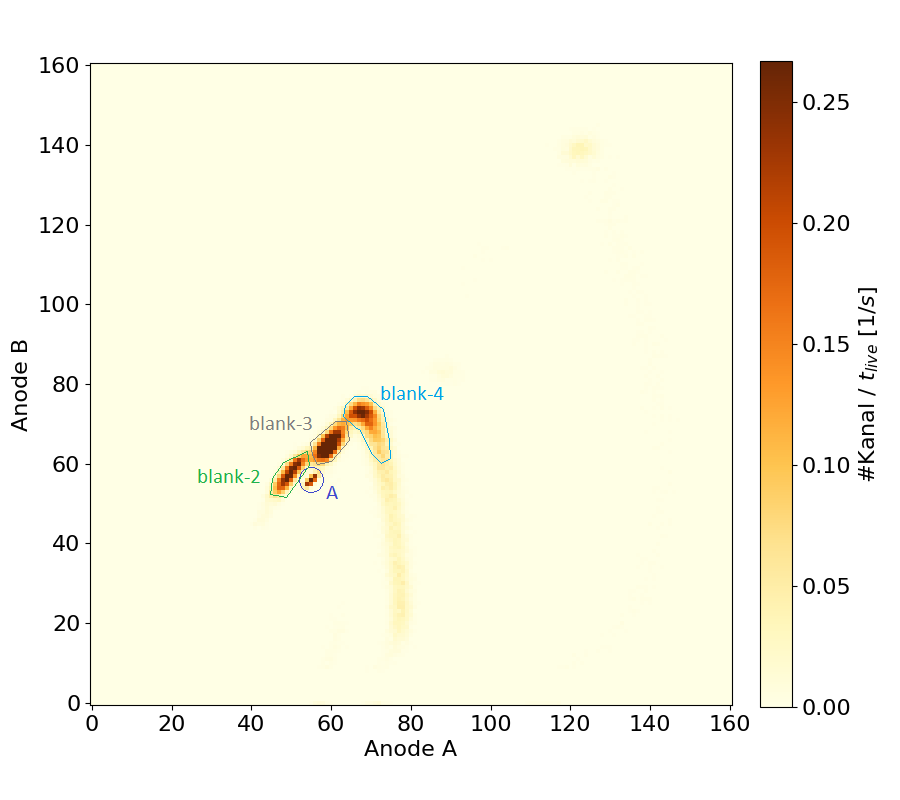
\includegraphics[width=\linewidth]{Pictures/Gasdetektor/3_blank_AB.png}
    \end{subfigure}
    \begin{subfigure}{0.47\textwidth}
        \centering
        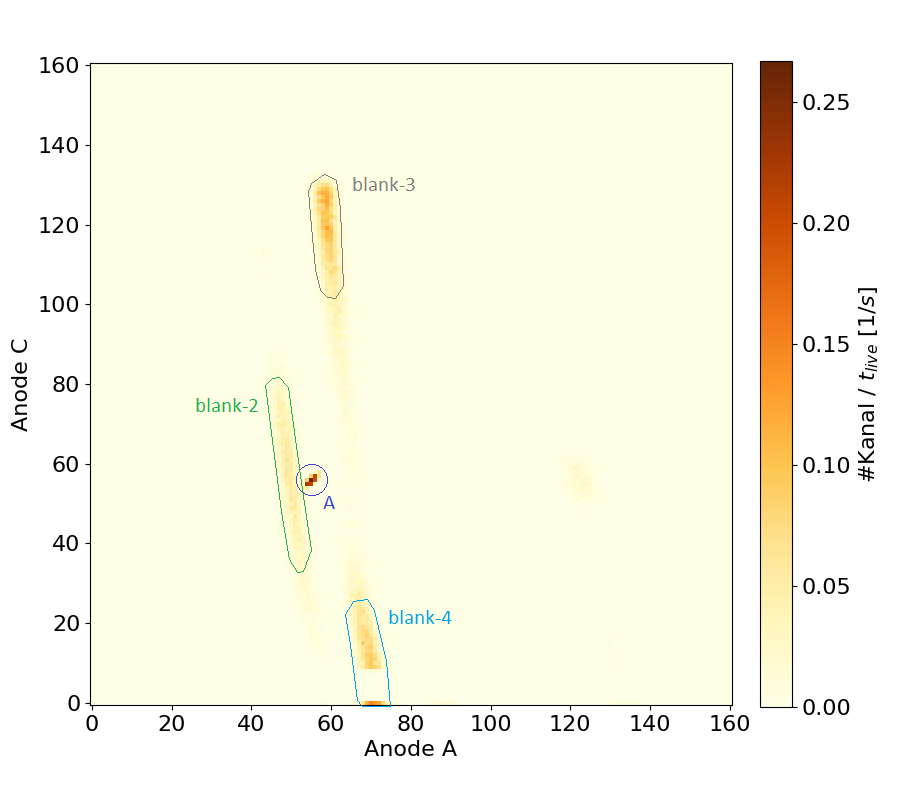
\includegraphics[width=\linewidth]{Pictures/Gasdetektor/3_blank_AC.png}
    \end{subfigure}
    \begin{subfigure}{0.47\textwidth}
        \centering
        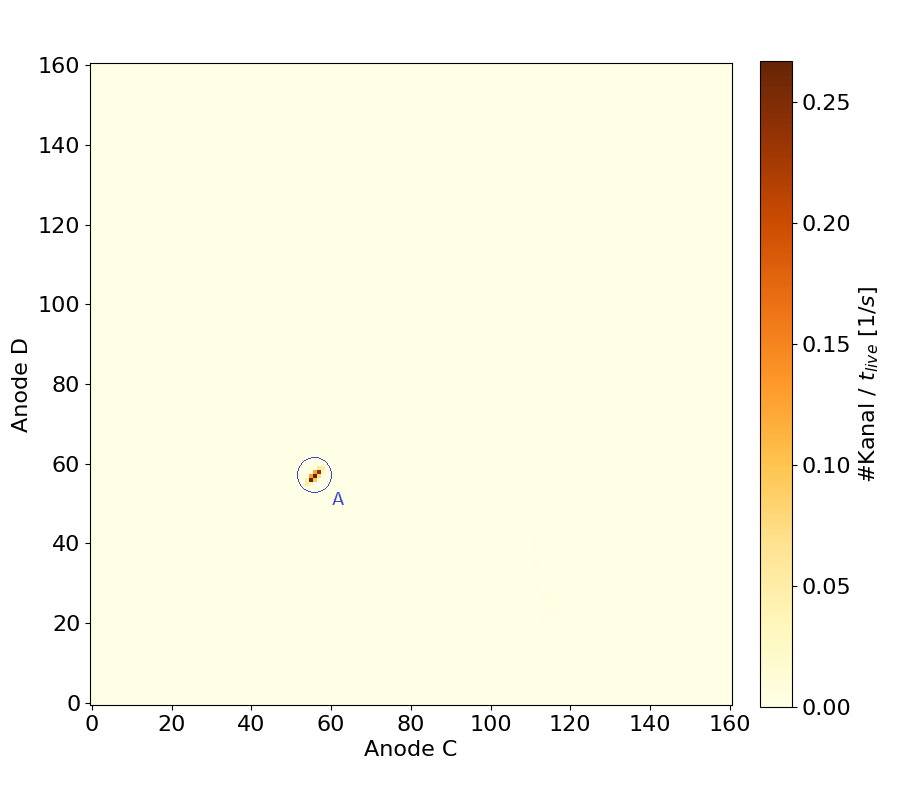
\includegraphics[width=\linewidth]{Pictures/Gasdetektor/3_blank_CD.png}
    \end{subfigure}
    \caption{2D-Spektren der Anoden in der Gasionisationskammer ohne Probe, live-Zeit von $t_{\text{live}} = \SI{1245}{\second}$}
    \label{Auswertung_Gasdetektor_2DSpektren_blank}
\end{figure}
\begin{figure}[H]
    \centering
    \begin{subfigure}{0.47\textwidth}
        \centering
        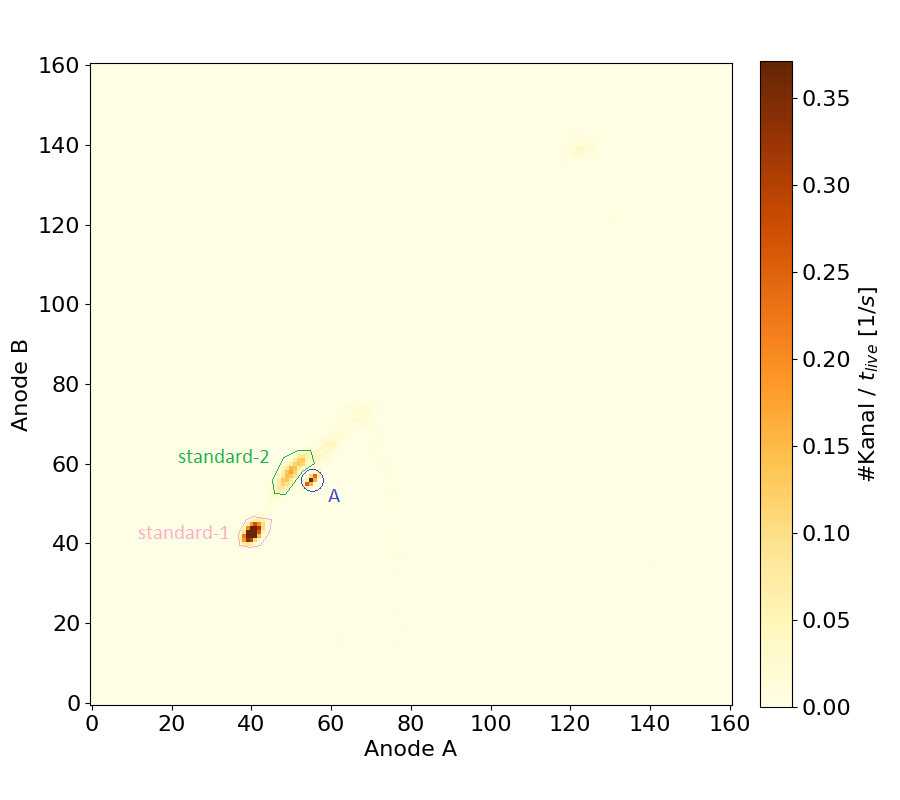
\includegraphics[width=\linewidth]{Pictures/Gasdetektor/22_standard_AB.png}
    \end{subfigure}
    \begin{subfigure}{0.47\textwidth}
        \centering
        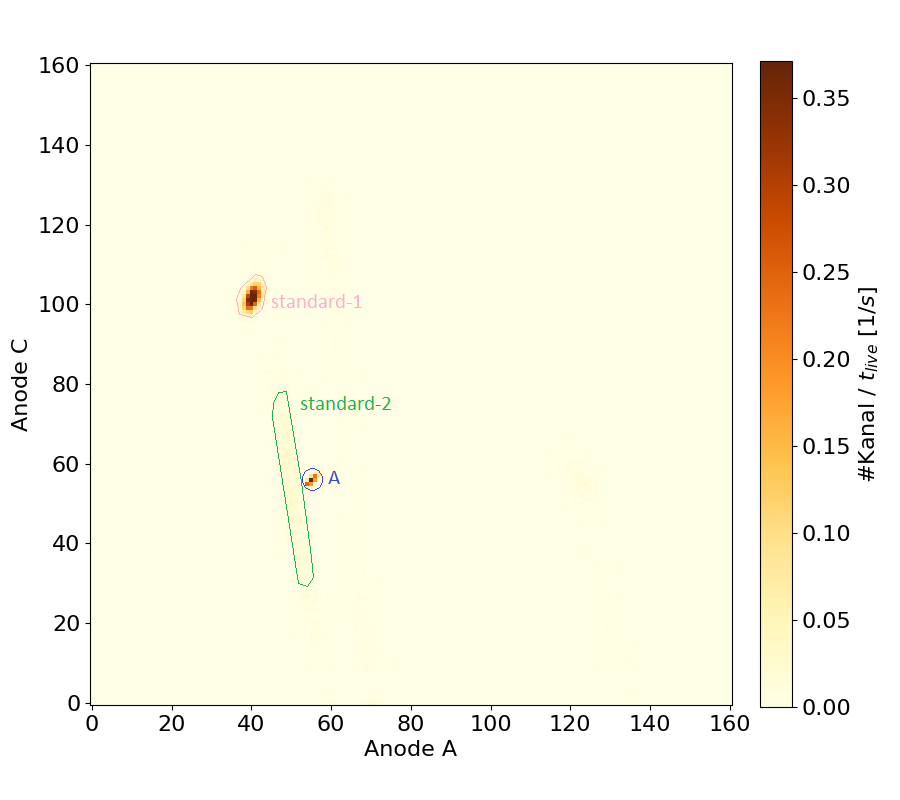
\includegraphics[width=\linewidth]{Pictures/Gasdetektor/22_standard_AC.png}
    \end{subfigure}
    \begin{subfigure}{0.47\textwidth}
        \centering
        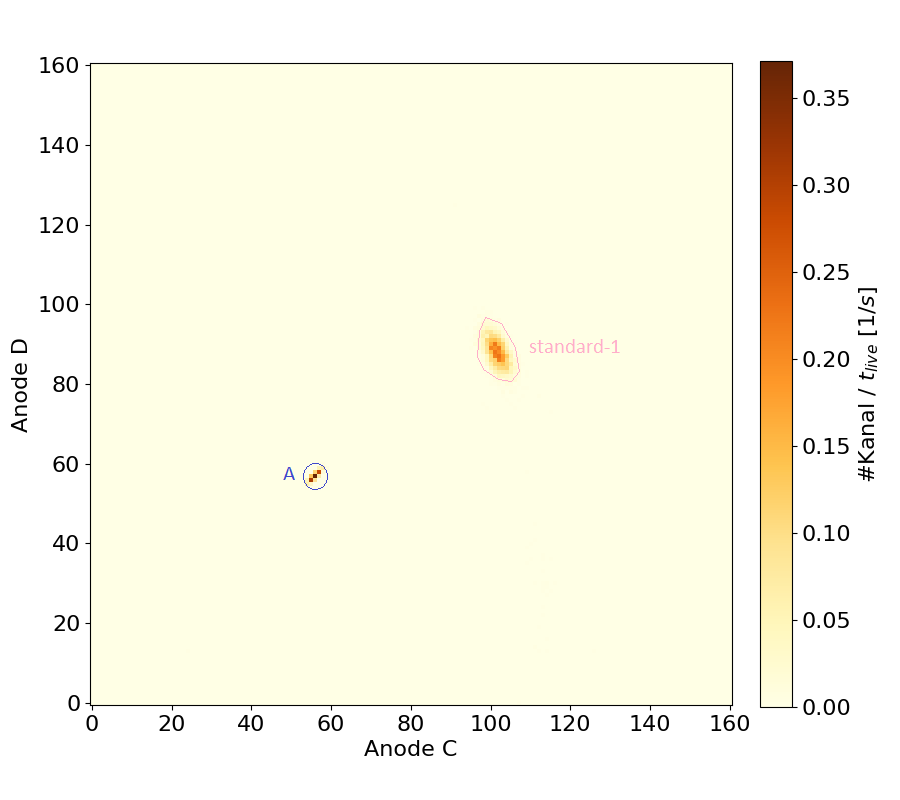
\includegraphics[width=\linewidth]{Pictures/Gasdetektor/22_standard_CD.png}
    \end{subfigure}
    \caption{2D-Spektren der Anoden in der Gasionisationskammer mit BeO-Probe, live-Zeit von $t_{\text{live}} = \SI{474}{\second}$}
    \label{Auswertung_Gasdetektor_2DSpektren_BeO}
\end{figure}
\begin{figure}[H]
    \centering
    \begin{subfigure}{0.47\textwidth}
        \centering
        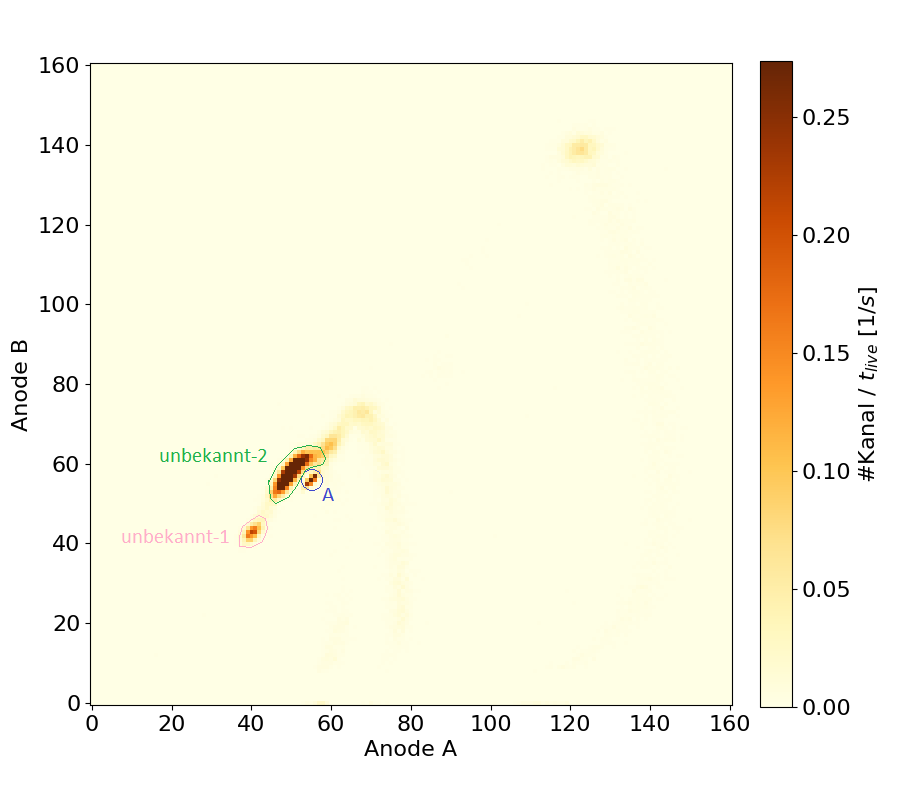
\includegraphics[width=\linewidth]{Pictures/Gasdetektor/19_probe_AB.png}
    \end{subfigure}
    \begin{subfigure}{0.47\textwidth}
        \centering
        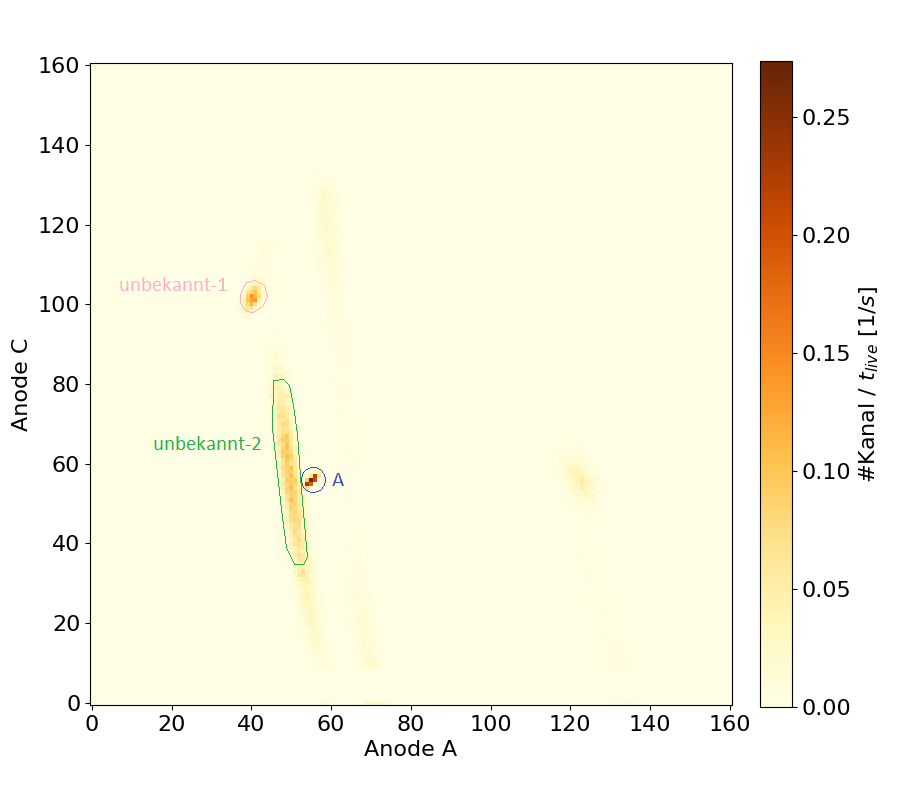
\includegraphics[width=\linewidth]{Pictures/Gasdetektor/19_probe_AC.png}
    \end{subfigure}
    \begin{subfigure}{0.47\textwidth}
        \centering
        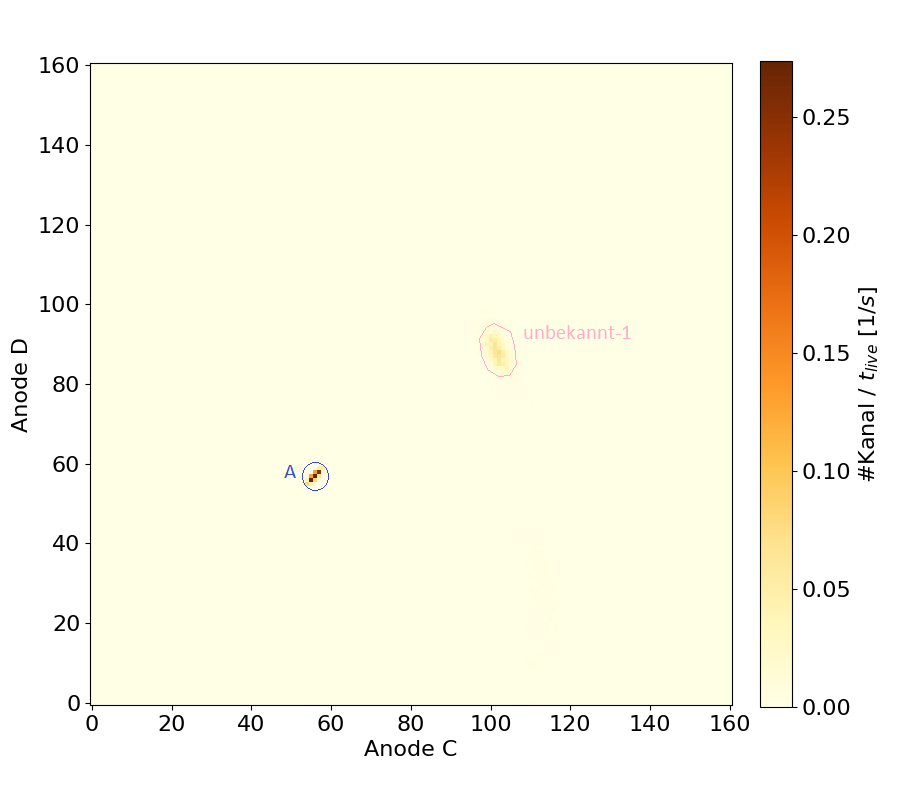
\includegraphics[width=\linewidth]{Pictures/Gasdetektor/19_probe_CD.png}
    \end{subfigure}
    \caption{2D-Spektren der Anoden in der Gasionisationskammer mit unbekannter Probe, live-Zeit von $t_{\text{live}} = \SI{845}{\second}$}
    \label{Auswertung_Gasdetektor_2DSpektren_unbekannt}
\end{figure}
Um die Markierten Bereiche etwas besser zu verstehen sind im Folgenden noch zwei TRIM-Simulationen visualisiert, bei denen die Ionisierung des Isobutan über der Eindringtiefe zweier Ionen aufgetragen ist:
\begin{figure}[H]
    \centering
    \begin{subfigure}[t]{0.47\textwidth}
        \centering
        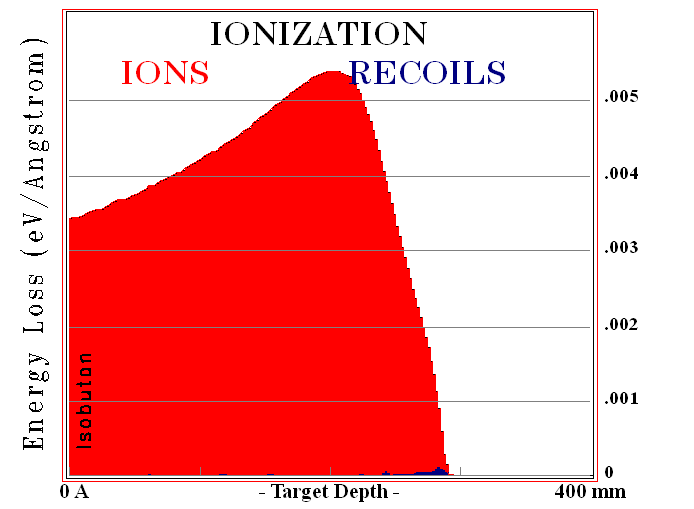
\includegraphics[height=0.25\textheight]{Pictures/TRIM_Ionisierung_10Be_in_Isobutan_vorher_2+.png}
        \caption{TRIM-Simulation für die Ionisierung von Isobutan durch $^{10}\text{Be}$, mit Anfangsenergie $E_{\text{Ion, Start}} = \SI{11.67}{\mega\electronvolt}$ (vor Folie $^{10}\text{Be}^{2+}$)}
        \label{Auswertung_Gasdetektor_TRIM_sims_Be}
    \end{subfigure}
    \begin{subfigure}[t]{0.47\textwidth}
        \centering
        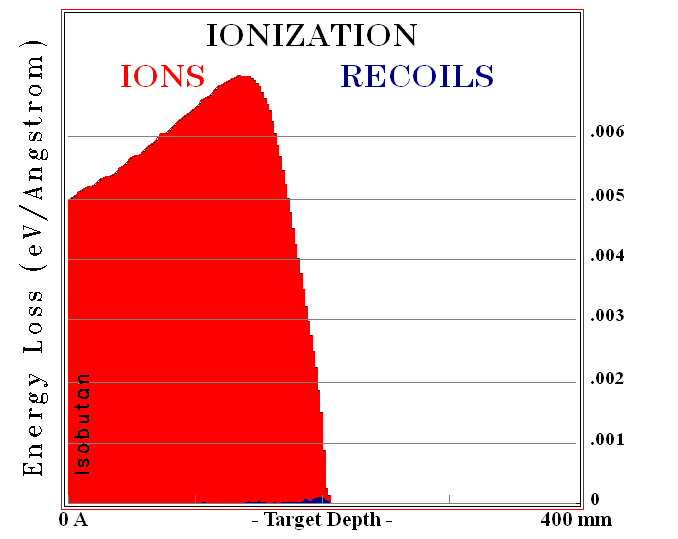
\includegraphics[height=0.25\textheight]{Pictures/TRIM_Ionisierung_10Bor_in_Isobutan_vorher_2+.png}
    	\caption{TRIM-Simulation für die Ionisierung von Isobutan durch $^{10}\text{B}$, mit Anfangsenergie $E_{\text{Ion, Start}} = \SI{11.30}{\mega\electronvolt}$ (vor Folie $^{10}\text{B}^{2+}$)}
        \label{Auswertung_Gasdetektor_TRIM_sims_B}
    \end{subfigure}
    \caption{TRIM-Simulationen für die Ionisierung von Isobutan durch $^{10}\text{Be}$ und $^{10}\text{B}$, wenn sie jeweils nach dem Beschleuniger den Ladungszustand $2+$ und nach der SiN-Folie den Ladungszustand $4+$ haben. Dies sind die einfachsten Fälle von Ionen, die es (möglicherweise) in den Detektor schaffen. Da bei Bor keine Ionisierung im Bereich ab \SI{20}{\centi\metre} stattfindet ist zu erwarten, dass Bor nicht in Spektren auftritt die die C- und D-Anode übereinander auftragen, solange das Bor mit der Anfangsenergie $E_{\text{Ion, Start}} = \SI{11.30}{\mega\electronvolt}$ eintrifft.}
    \label{Auswertung_Gasdetektor_TRIM_sims}
\end{figure}
Die Fläche unter den Ionisierungskurven bis zu einer bestimmten Eindringtiefe bestimmt den Ort des Ions in den 2-D-Spektren.

Fangen wir bei der Auswertung mit den Gemeinsamkeiten der Spektren an.
Für die Auswertung wurden ähnliche Bereiche in den Spektren mit den selben Nummern und Farben versehen.
Man kann die selbe Teilchenspezies über zwei Spektren hinweg miteinander identifizieren, da immer mindestens eine Achse zwischen den Spektren geteilt ist, und Spezies auf einer Achse (wenn überhaupt) in jedem Spektrum in dem selben Wertebereichen stehen müssen.
Daher sind die Farben und Nummern in allen Spektren geteilt, und man sieht das im wesentlichen fünf verschiedene Spezies identifiziert werden müssen.
Dabei muss nicht jedes ein neues Nuklid sein, es kann sich auch um ein schon gefundenes Nuklid handeln, welches aber eine andere Anfangsenergie besitzt.

Zuerst schauen wir uns die bekannte BeO-Probe in Abb. \ref{Auswertung_Gasdetektor_2DSpektren_BeO} an.
Da wir in der BeO-Probe davon ausgehen können eine sehr reine Probe zu haben, ist der Bereich 1 (pink) eindeutig dem Nuklid $^{10}Be$ zuzuordnen, denn es tritt am häufigsten auf und es wird in allen Spektren in sinnvollen Kanälen gefunden (Kanäle entsprechen dabei dem Strom, und damit der Energie die an einer Anode ankam).
Man kann also davon ausgehen, dass dieses $^{10}\text{Be}$ aus der Probe als $^{10}\text{Be}^{16}\text{O}^{1-}$ gelöst wurde.
Im Tandembeschleuniger ist der Sauerstoff abgespalten und $^{10}\text{Be}^{2+}$ wurde weiter beschleunigt.
In der SiN-Folie wurde es schließlich Umgeladen zu $^{10}\text{Be}^{4+}$, als welches es schließlich in den Detektor gefallen ist.
Da wir die Kalibrierung der ESA und der Ablenkmagnete genau auf diesen Prozess eingerichtet haben hat es kein Problem den Detektor zu erreichen.

Kniffliger wird es bei Spezies 2 (grün), denn diese wird ebenfalls in der reinen BeO-Probe gefunden, jedoch findet man sie dort nicht im Spektrum der letzten beiden Anoden.
Sie schafft es jedoch bis zur Anode C, das heißt sie wird in dieser Detektortiefe vollständig gestoppt.
Da sie schon im Spektrum von Anode A und B erkennbar mehr Energie verliert als Spezies 1, jedoch im Spektrum von Anode A und C unter der Spezies 1 liegt und damit dort weniger Energie abgibt, und wegen der reinen BeO-Probe, liegt es nahe, dass es sich hier auch um Beryllium handelt.
Denn wenn dieses eine niedrigere Energie bei Eintritt in den Detektor (im Vergleich mit Spezies 1) mitbringt ist genau dieses Verhalten zu erwarten.
Der beste Kandidat für diese Spezies ist $^{9}\text{Be}$, denn dieses kann als $^{9}\text{Be}^{16}\text{O}^{1}\text{H}^{1-}$ aus der Probe gelöst werden, kann sich dann im Tandem vom $^{16}\text{O}$ trennen und dann als Isobar $^{9}\text{Be}^{1}\text{H}^{2+}$ bis zur SiN-Folie bewegen.
Das $^{9}\text{Be}^{16}\text{O}^{1}\text{H}^{1-}$ im Tandem nicht auch den Wasserstoff verliert ist unwahrscheinlich.
Dies erklärt immerhin teilweise die geringe Intensität der Spezies in dem Spektrum von BeO (im Vergleich zu $^{10}\text{Be}$, welches sonst deutlich seltener wäre).
Beim Eintritt in die dichte Folie trennen sich $^{9}\text{Be}$ und $^{1}\text{H}$.
Das $^{9}\text{Be}$ verbleibt mit $\frac{9}{10}$ der kinetischen Energie des Ions nach dem Beschleuniger (\SI{11.27}{\mega\electronvolt}).
Dann wird es in der SiN-Folie abgebremst.
Hier wurde wieder SRIM/TRIM benutzt.
Die Energie nach der Folie ist dann \SI{10.42}{\mega\electronvolt}, die Spezies ist $^{9}\text{Be}^{4+}$.
Damit hat es ca. \SI{89}{\percent} der Energie, die ein $^{10}\text{Be}^{4+}$ an dieser stelle hätte, also wie gesucht weniger.
Weitere SRIM/TRIM-Simulationen zeigen, dass es mit dieser Energie eine Eindringtiefe von \SI{254}{\milli\metre} im Detektor hätte, also würde es auch Anode D erreichen.
Was hier jedoch noch fehlt, ist das das Ion aufgrund seiner geringeren kinetischen Energie und Masse nicht ohne Probleme durch den HE-ESA und den vertikalen Ablenkmagneten kommt.
Im ESA führt dies zu einer stärkeren Ablenkung (nach Gleichung \ref{Auswertung_Formel_ESA} ist für diesen Fall der Krümmungsradius der Trajektorie proportional zur kinetischen Energie des Ions), im vertikalen Ablenkmagneten ebenfalls zu einer stärkeren (Gleichung \ref{Auswertung_eq_Magnet}, Krümmungsradius proportional zu $\sqrt{m_{\text{Ion}}E_{\text{kin}}}$).
Da die Ablenkungen senkrecht zueinander stehen sind sie quasi unabhängig voneinander.
Es liegt hier nahe, dass das Ion noch Energie verliert wenn es mit dem inneren des Strahlrohrs kollidiert.
Da der Auftreffwinkel aber klein ist verliert es nicht alle Energie, wie viele andere Ionen.
Ein bisschen ausprobieren in TRIM hat gezeigt, dass $^{9}\text{Be}^{4+}$ unterhalb von etwa \SI{8.5}{\mega\electronvolt} Eintrittsenergie nicht mehr die Anode D erreicht.
Da wir den genauen Aufbau nicht kennen, können wir nicht abschätzen, ob so ein Energieverlust realistisch ist.
Dies würde jedoch nicht nur die das Fehlen des Ions im letzten Spektrum erklären, sondern auch warum der Fleck in den anderen Spektren so viel breiter ist als der der ersten Spezies, denn Stöße sind stochastische Prozesse, was unweigerlich zu so einer "Verschmierung" der Energie führt.

Um dieses Argument noch etwas zu bekräftigen wollen wir uns als nächstes die Spektren in Abbildung \ref{Auswertung_Gasdetektor_2DSpektren_blank} ansehen, bei denen gar keine Probe verwendet wurde.
Auch dort ist diese 2. Spezies zu identifizieren, was für das stabile und häufig vorkommende $^{9}\text{Be}$-Isotop spricht.
Als nächstes wollen wir uns mit den Spezies 3 (grau) und 4 (blau) beschäftigen.
Auch hier fällt auf, dass die Ionen nicht die Anode D erreichen können.
Hier werden beide als $^{10}\text{B}$ identifiziert.
In beiden Fällen handelte es sich nach dem Beschleuniger um $^{10}\text{B}^{2+}$.
Auch hier ist die Begründung im wesentlichen eine Energieverlust durch Kollisionen mit dem Strahlrohr (ohne die selben Argumente nocheinmal anzuführen).
Dennoch gibt es Unterschiede.
So kann man der Spezies 3 das Ion $^{10}\text{B}^{4+}$ nach der SiN-Folie zuordnen.
Da es nach der SiN-Folie eine Energie von \SI{11.30}{\mega\electronvolt} ist der Krümmungsradius der Trajektorie im HE-ESA und im vertikalen Ablenkmagneten nicht viel anders als der von $^{10}\text{Be}^{4+}$, jedoch genug um Kollisionen mit dem Strahlrohr zu verursachen und damit eine Aufweichung des Flecks im Spektrum hervorzurufen.
Der Spezies 4 kann das Ion $^{10}\text{B}^{3+}$ nach der SiN-Folie zugeordnet werden.
Dies führt dazu, dass der Krümmungsradius der Trajektorien in beiden Ablenkern am Ende überproportional größer wird (denn beide sind proportional zum inversen der Ladung).
Das Ion kollidiert dann genau mit der anderen Seite des Strahlgangs.
Am Ende hat Spezies 4 die geringste Energie wenn sie in den Detektor kommt, und einige der Ionen schaffen es nicht mal bis zu Anode C, weshalb der Fleck im A-C-Spektrum nach unten etwas abgeschnitten ist.

Als letztes bleibt die Spezies, die in den Spektren mit "A" betitelt wurde.
Hierbei handelt es sich offenbar um Ionen mit einer derart hohen Energie, dass sie den Detektor einfach passieren.
Ferner ist ihr Energieverlust in allen Berechen des Detektors immer fast konstant, was ebenfalls für eine sehr große kinetische Energie spricht, denn Ionen verlieren in den hier betrachteten Energiebereichen immer die meiste Energie in Materie, wenn sie schon fast stehen.
Da kein "Fingerabdruck" im Detektor hinterlassen wird ist eine Identifikation hier nicht möglich.

Schauen wir zum Abschluss noch auf Abbildung \ref{Auswertung_Gasdetektor_2DSpektren_unbekannt}, Spektren einer unbekannte Probe.
Durch die vorherigen Erkenntnisse lassen sich schnell die Teilchenspezies 1 und 2 erkennen.
Es handelt sich bei der Probe also um ein Berylliumhaltiges, aber nicht sehr Borhaltiges Material (schwach sind auch Spezies 3 und 4 zu erkennen).
Die Signaturen sind hier genau die selben.
Nur die Intensitäten der Spezies sind im vergleich zur bekannten BeO-Probe vertauscht (qualitativ).
Diese Probe enthält also verhältnismäßig mehr $^{9}\text{Be}$ und weniger $^{10}\text{Be}$.
Genaue Zahlenwerte sind ohne die Referenzwerte der BeO-Probe nicht anzugeben, aber eine solche Konzentrationsbestimmung wird dafür beispielhaft in der nächsten Aufgabe durchgeführt.
